\usetikzlibrary{arrows, positioning, automata}

\newlength{\circleheight}
\setlength{\circleheight}{1.5cm}
\newlength{\circlewidth}
\setlength{\circlewidth}{3.4cm}
\newlength{\horseplength}
\setlength{\horseplength}{8cm}
\newlength{\verseplength}
\setlength{\verseplength}{6cm}

\newcommand{\initialgastext}{\centering \textbf{Interstellar gas} \\ Characterized by initial mass function of stars that will form}
\newcommand{\starformationtext}{\centering \textbf{Star formation} \\ Collapse of initial gas into stars \\ Characterized by the star formation rate}
\newcommand{\stardeathtext}{\centering \textbf{Death of stars} \\ Explosive ejection of enriched gas \\ Characterized by isotopic yield tables}
\newcommand{\inflowtext}{\centering \textbf{Inflow} \\ Prestine gas from extragalactic medium}
\newcommand{\outflowtext}{\centering \textbf{Outflow} \\ Enriched gas ejected from intergalactic medium}

\centering
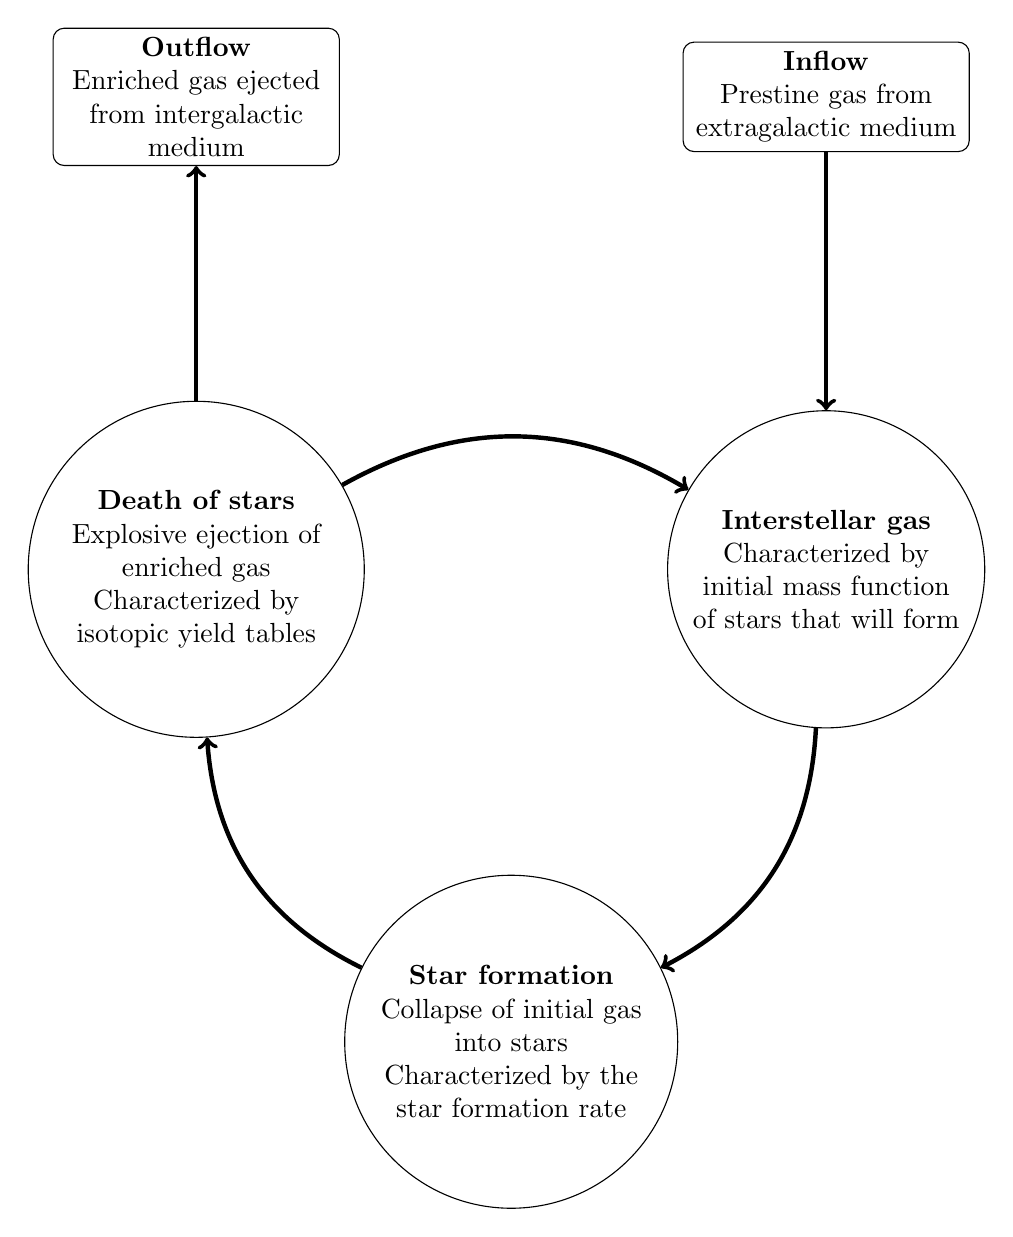
\begin{tikzpicture}[bubble/.style={circle, draw}, flow/.style={rounded corners, draw}]
  %Make nodes with circles of text
  \draw (0.5\horseplength,\verseplength) node[bubble] (A) {\parbox{\circlewidth}{\initialgastext}};
  \draw (0,0) node[bubble] (B) {\parbox{\circlewidth}{\starformationtext}};
  \draw (-0.5\horseplength,\verseplength) node[bubble] (C) {\parbox{\circlewidth}{\stardeathtext}};
  \draw (0.5\horseplength, 2\verseplength) node[flow] (D) {\parbox{\circlewidth}{\inflowtext}};
  \draw (-0.5\horseplength, 2\verseplength) node[flow] (E) {\parbox{\circlewidth}{\outflowtext}};

  %curved arrows between bubbles
  \path (A) edge[bend left, ->, ultra thick] (B);
  \path (B) edge[bend left, ->, ultra thick] (C);
  \path (C) edge[bend left, ->, ultra thick] (A);
  \path (D) edge[->, ultra thick] (A);
  \path (C) edge[->, ultra thick] (E);
\end{tikzpicture}
\caption[Stellar enrichment diagram]{\label{tikz:stellar-enrichment}
  Diagram depicting recycling of gas in a one-zone galaxy model.
  Initially the stellar gas is prestine, from big bang nucleosynthesis, just like the inflow from extragalactic gas.
  Stars form from the prestine gas, forming stellar populations from a given star formation rate and initial mass function.
  Stars end their life asymptotic giant branch stars or explosive type 2 supernovae, ejecting enriched material back into the interstellar medium.
  These events leave remnants, like white dwarves, neutron stars and black holes, which can interact with eachother and other stars to produce secondary explosive events.
  Together the explosive events can drive additional outflow of enriched material away from the galaxy, into the extragalactic medium.
  It should noted that this applies to one-zone models of galaxies, which have two sides; the inside and the outside.
  Ignoring all effects from layered structure of galaxies like; circumgalactic medium, disk, bulge, etc.
}
